\chapter{Das LHCb-Experiment}  \label{kap:experiment}
Der Large Hadron Collider (LHC) am Kernforschungszentrum CERN in Genf ist der derzeit größte Ringbeschleuniger der Erde. Er hat einen Durchmesser von ca. $27\kilo\meter$. Im Ring werden zwei geladene Teilchenstrahlen in gegenläufiger Richtung auf nahezu Lichtgeschwindigkeit beschleunigt und anschließend an vier möglichen Punkten zur Kollision gebracht. Bei den Teilchenstrahlen handelt es sich hauptsächlich um Protonenstrahlen, es werden aber auch Proton-Blei- und Blei-Blei-Kollisionen untersucht. An den vier Kollisionspunkten sind die großen Experimente positioniert: ATLAS, CMS, ALICE und LHCb. Eine der Hauptaufgaben der Experimente ATLAS und CMS ist die Suche nach dem Higgs-Boson, ALICE hingegen untersucht das Quark-Gluon-Plasma. Im folgenden soll nun aber detailliert auf das LHCb-Experiment eingegangen werden. \cite{lhc-info}

\section{Aufgaben und Ziele des Experimentes}
Während des Urknalls sind Materie und Antimaterie in gleicher Zahl entstanden. Treffen ein Teilchen und ein Antiteilchen aufeinander, so werden diese vernichtet und es wird Energie frei. Doch wenn zunächst gleich viel Materie und Antimaterie vorhanden war, verwundert es, warum das Universum nur aus Materie besteht und überhaupt noch existiert.

Das Standardmodell der Teilchenphysik kann dieses Ungleichgewicht nur unzureichend erklären. Es beschreibt zwar die \CP-Verletzung der schwachen Wechselwirkung, die auch Bestandteil dieser Arbeit ist, und liefert damit einen potentiellen Kandidaten zur Erklärung, allerdings ist jene zu schwach. Es muss also auch \CP-verletzende Beiträge jenseits des Standardmodells geben, die evtl. durch noch nicht beobachetete Teilchen berursacht werden. An dieser Stelle setzt LHCb an. Es untersucht Teilchen und Zerfälle, die von einem $b$- bzw. $\overline{b}$-Quark (außerdem auch $c/\overline{c}$-Quarks) ausgehen. Aus diesen bilden sich B-(D-)Mesonen, die sehr sensitiv auf Hinweise für \glqq neue Physik\grqq\ sind. Diverse Zerfalls- und Mischprozesse dieser Mesonen enthalten in ihren dazugehörigen Feynmangraphen Schleifen (in \glqq Pinguin-\grqq bzw. Box-Diagrammen), in denen es möglich ist, dass neben dem Standardmodell auch \glqq neue Physik\grqq\ Beiträge zu Zerfallsamplituden etc. liefert. In diesen Schleifen darf nach Heisenberg die Energieerhaltung kurzzeitig verletzt werden, sodass sie virtuelle Teilchen mit einer Masse deutlich über der vorhandenen Schwerpunktsenergie enthalten kann. Man versucht also indirekt (über Schleifenbeiträge) Hinweise auf neue Teilchen und Prozesse zu finden. Um dies erfolgreich zu gestalten, ist eine präzise Messung des Standardmodells unabdingbar. \cite{cern-courier, roadmap, lhcb-info}

\section{Der LHCb-Detektor}
Im Gegensatz zu den anderen Experimenten ist der LHCb-Detektor ein einarmiges Vorwärtsspektrometer. Dies liegt daran, dass $b\overline{b}$-Paare hauptsächlich in oder entgegen der Protonenstrahlrichtung produziert werden. Aus Kostengründen hat man darauf verzichtet, den Detektor in Vorwärts- und Rückwärtsrichtung zu bauen. Stattdessen lag der Fokus darauf, nur einen Detektor, aber mit entsprechend besserer Präzision und Auflösung zu bauen. Abbildung \ref{fig:detektor} zeigt einen Schnitt durch die (y,z)-Ebene des Detektors. Der Detektor deckt in x-Richtung einen Bereich von $10-300\milli\rad$ und in y-Richtung von $10-250\milli\rad$ ab. Die Subdetektoren lassen sich nach ihrem Zweck in zwei Unterkategorien einteilen: Detektoren zur Spurrekonstruktion und zur Teilchenidentifikation.

\begin{figure}[hptb]
\centering
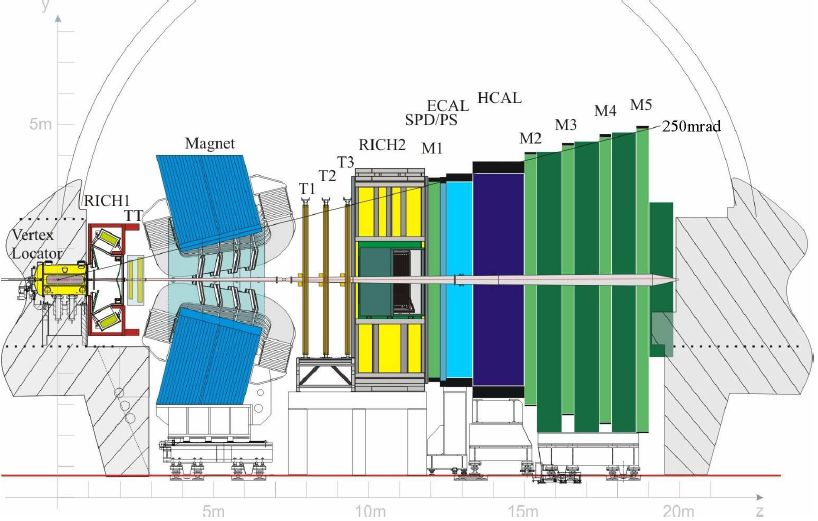
\includegraphics[width=\textwidth]{detektor}
\caption{Schnitt durch die (y,z)-Ebene des LHCb-Detektors. Die Abbildung wurde \cite{detector} entnommen.}
\label{fig:detektor}
\end{figure}


\subsection{Spurdetektoren}
Hauptaufgabe der Spurdektektoren ist die Impulsbestimmung geladener Teilchen. Dazu werden diese durch das Feld eines Dipolmagneten abgelenkt. Die Trajektorien werden mit den Stationen VELO, TT und T1-T3 gemessen, die im Folgenden detaillierter beschrieben werden. Die Ablenkung des Teilchens von seiner ursprünglichen Trajektorie gibt Aufschluss über den Impuls. Das Magnetfeld ist weitestgehend homogen mit einer dominierenden y-Komponente, sodass die Ablenkung hauptsächlich in der (x,z)-Ebene vonstattengeht. Über die Länge $l=10\meter$ integriert beträgt die Feldstärke $\int B\mathrm{d}l = 4\tesla\meter$. Um ladungsabhängige Detektorasymmetrien zu messen, kann die Orientierung des Magnetfeldes umgekehrt werden. \cite{thesis_linn}

\subsubsection{Vertex Locator (VELO)}
Aufgabe des Vertex Locator (VELO) ist die Detektion des Primärvertex (Entstehung eines Teilchens) sowie des Sekundärvertex (erste Interaktion des Teilchens, meist Zerfall). Er ist sehr nah am Kollisionspunkt aus Silikonstreifen aufgebaut und besteht aus 21 Stationen. Um Schäden zu vermeiden, besteht der VELO aus zwei Hälften, die erst zusammengeführt werden, sobald der Teilchenstrahl im Experiment stabil ist.

\subsubsection{Tracker Turicensis (TT)}
Der Tracker Turicensis (TT) besteht aus zwei Stationen, die sich hinter dem Magneten befinden und eine Detektionsfläche von etwa $8,4\meter^2$ bieten. Sie sind wie der VELO aus Silikonstreifen aufgebaut und ermöglichen eine dreidimensionale Spurrekonstruktion, wobei die TT-Stationen so aufgebaut sind, dass die Präzision in der horizontalen Ablenkungsebene (x,z) des Magneten am besten ist. Die Auflösung eines einzelnen Teilchentreffers beträgt etwa $50\micro\meter$.

\subsubsection{Inner Tracker (IT)}
Im Zentrum der drei Stationen T1-T3 nach dem Dipolmagneten ist der sogenannte Inner Tracker platziert. Er ist $120\centi\meter$ breit und $40\centi\meter$ hoch, ebenfalls ein Silikonstreifendetektor und besteht aus vier Schichten, die ähnlich wie die TT Stationen aufgebaut sind. Er deckt eine Fläche von etwa $4\meter^2$ ab und erzielt ebenfalls eine Trefferauflösung von $50\micro\meter$.

\subsubsection{Outer Tracker (OT)}
Der Outer Tracker bildet den äußeren Teil der Stationen T1-T3, der nicht vom IT abgedeckt wird. Er besteht ebenfalls aus 4 Schichten und ist aus Driftröhrchen aufgebaut, die mit einem Gasgemisch aus Argon (70\%), CO$_2$(28,5\%) und O$_2$ (1,5\%) gefüllt sind. Im Innern der Röhrchen verläuft ein mit Gold beschichteter Anodendraht aus Wolfram. Die räumliche Auflösung eines einzelnen Röhrchens liegt bei $200\micro\meter$.

\subsubsection{Klassifizierung von Spuren} \label{kap:spurklassen}
Je nachdem, welche Detektoren getroffen wurden, teilt man die Spuren in vier unterschiedliche Kategorien ein:
\begin{itemize}
\item \textbf{VELO Spuren} enthalten Treffer ausschließlich im VELO und dienen hauptsächlich der Rekonstruktion des Primärvertex.
\item Hinterlassen die Teilchen Treffer im VELO und in den TT-Stationen, spricht man von \textbf{Upstream Spuren}. Hierbei handelt es sich dann um Teilchen mit kleinem Impuls, da der Magnet die Teilchen so stark ablenkt, dass jene den Akzeptanzbereich des Detektors verlassen und die anschließenden Detektoren nicht mehr passieren.
\item Bei \textbf{Downstream Spuren} gibt es nur Treffer in den Stationen TT und T1-T3. Diese treten vor allem bei langlebigen Teilchen wie dem $\Kshort$ auf, die den VELO vor ihrem Zerfall verlassen. In dieser Arbeit werden ausschließlich Downstream Spuren verwendet (siehe dazu auch Kapitel \ref{kap:downstream})
\item Gibt es Treffer in allen Stationen (VELO, TT, T1-T3), so spricht man von \textbf{Long Spuren}. Da es hier die meisten Treffer gibt, haben diese Spuren die präziseste Impulsauflösung. \cite{thesis_linn}
\end{itemize}

\subsection{Detektoren zur Teilchenidentifikation}
Neben der Rekonstruktion der Spuren ist es natürlich essentiell, auch die Teilchen zu identifizieren. Hierzu werden die Informationen der Detektoren RICH1/2, SPD, PS HCAL, ECAL sowie M1-M5 für eine Teilchenhypothese verwendet.

\subsubsection{Die Ring Imaging Cherenkov Detektoren (RICH)}
Die beiden RICH Detektoren nutzen die Cherenkov-Strahlung, um Teilchen voneinander zu unterscheiden, insbesondere $\pi^{\pm}$ und $K^{\pm}$. Ähnlich dem Machschen Kegel bei Schall emittieren geladene Teilchen Photonen in Kegelform, wenn sie ein Medium mit einer Geschwindigkeit $v$ passieren, die größer ist als die Lichtgeschwindigkeit $c'=c/n$ in diesem Medium ($n:$ Brechungsindex des Mediums). Für den Öffnungswinkel $\theta_{\text{C}}$ des Lichtkegels gilt dann:
\begin{align}
\cos \theta_{\text{C}} = \frac{c}{vn}.
\end{align}
Durch Messung des Öffnungswinkels und der Impulsinformation aus den Spurdetektoren lässt sich die Teilchenmasse bestimmen und somit eine Teilchenhypothese aufstellen. RICH1 ist dabei für kleine Impulse im Bereich von $1\giga\electronvolt$ bis $60\giga\electronvolt$ zuständig und deckt den kompletten Akzeptanzbereich des Detektors ab, RICH2 arbeitet dagegen bei Impulsen von $15\giga\electronvolt$ bis $100\giga\electronvolt$ und deckt einen Winkelbereich von ca. $15\milli\rad$ bis $120\milli\rad$ in horizontaler und $100\milli\rad$ in vertikaler Ebene ab.

\subsubsection{Kalorimetersystem}
Das Kalorimetersystem dient zur Identifikation von Elektronen, Photonen sowie Hadronen und soll deren Energie und Position bestimmen. Durch Wechselwirkung mit dem Kalorimetermaterial erzeugen jene einen kaskadenartigen Zerfall. Bei den Subdetektoren des Systems handelt es sich um Szintillationsdetektoren. Diese sind im Einzelnen:
\begin{itemize}
\item Der \textbf{Scintillating Pad Detector (SPD)} kann nur geladene Teilchen detektieren und dient damit der Unterscheidung von Photon und Elektron.
\item Auf den SPD und eine $12\milli\meter$ dicke Bleiplatte folgt der \textbf{Preshower Detector (PS)}. Die Platte löst Kaskaden von Photonen und Elektronen aus. Hadronische Kaskaden beginnen erst später und können damit unterschieden werden.
\item Das \textbf{elektromagnetische Kalorimeter (ECAL)} besteht im Wechsel aus Blei- und Szintillationsplatten und detektiert Photonen- und Elektronenschauer.
\item Beim \textbf{hadronischen Kalorimeter (HCAL)} wechseln sich Eisen- und Szintillationsplatten ab. Er ist sensitiv für hadronische Kaskaden.
\end{itemize}

\subsubsection{Myonkammern}
Der LHCb-Detektor besitzt insgesamt 5 Myonenkammern (M1-M5). Zur Verbesserung der Impulsmessung im Trigger ist M1 vor den Kalorimetern angebracht, die restlichen am Ende des Detektors. Zwischen M2-M5 befinden sich $80\centi\meter$ dicke Eisenplatten zur Absorption hadronischer Teilchen. Ab einem Impuls von etwa $6\giga\electronvolt/c$ können die Myonen alle 5 Stationen passieren. \cite{thesis_linn}

\subsection{Trigger}
Der LHCb-Detektor besitzt ein dreistufiges Triggersystem, um die Ereignisrate von $40\mega\hertz$ auf $2-3\kilo\hertz$ zu reduzieren. Die hierin enthaltenen Informationen werden dann zur weiteren Bearbeitung gespeichert. Die drei Stufen bestehen aus dem Hardwaretrigger \textbf{L0}, der die Ereignisrate auf $1\mega\hertz$ senkt, sowie den beiden software-basierten \glqq High Level Trigger\grqq\ \textbf{HLT1}($50\kilo\hertz$) und \textbf{HLT2}($2-3\kilo\hertz$). Für die Trigger siehe auch Kapitel \ref{kap:trigger}.